\documentclass[12pt]{article}

\usepackage{graphicx}
\usepackage{float}
\usepackage[a4paper, total={6in, 8.5in}]{geometry}

\setlength{\abovecaptionskip}{-10pt}

\title{Autocorrelation in Weather}

\author{Luke Swaby}

\date{October 2020}

\begin{document}
	\maketitle
  
	\begin{abstract}
	An investigation into temporal autocorrelation of weather conditions in Key West, Florida for the 20th century.
	\end{abstract}
  
	\section{Methodology}
	Two vectors of length $n-1$ (=99) were created of the temperatures of successive years in Key West, Florida for the 20th century, such that each element of the first vector (temperature in year $t$) corresponded in index to the temperature in the next time unit in the second vector (temperature in year $t+1$). 
	
	Pearson’s correlation coefficient was then computed between these two vectors, yielding a lag-1 autocorrelation value which was then compared against a vector of 10,000 likewise-computed autocorrelation coefficients for randomly permuted versions of the same temperature vector to obtain an approximate $p$-value.
	
	\section{Results}
	The autocorrelation coefficient calculated was 0.326 (3 d.p.), with an approximate $p$-value of $~0.0002$.
	
	\begin{figure}[H]
	\centering
	\vspace{-20mm} % A global option would be better here
	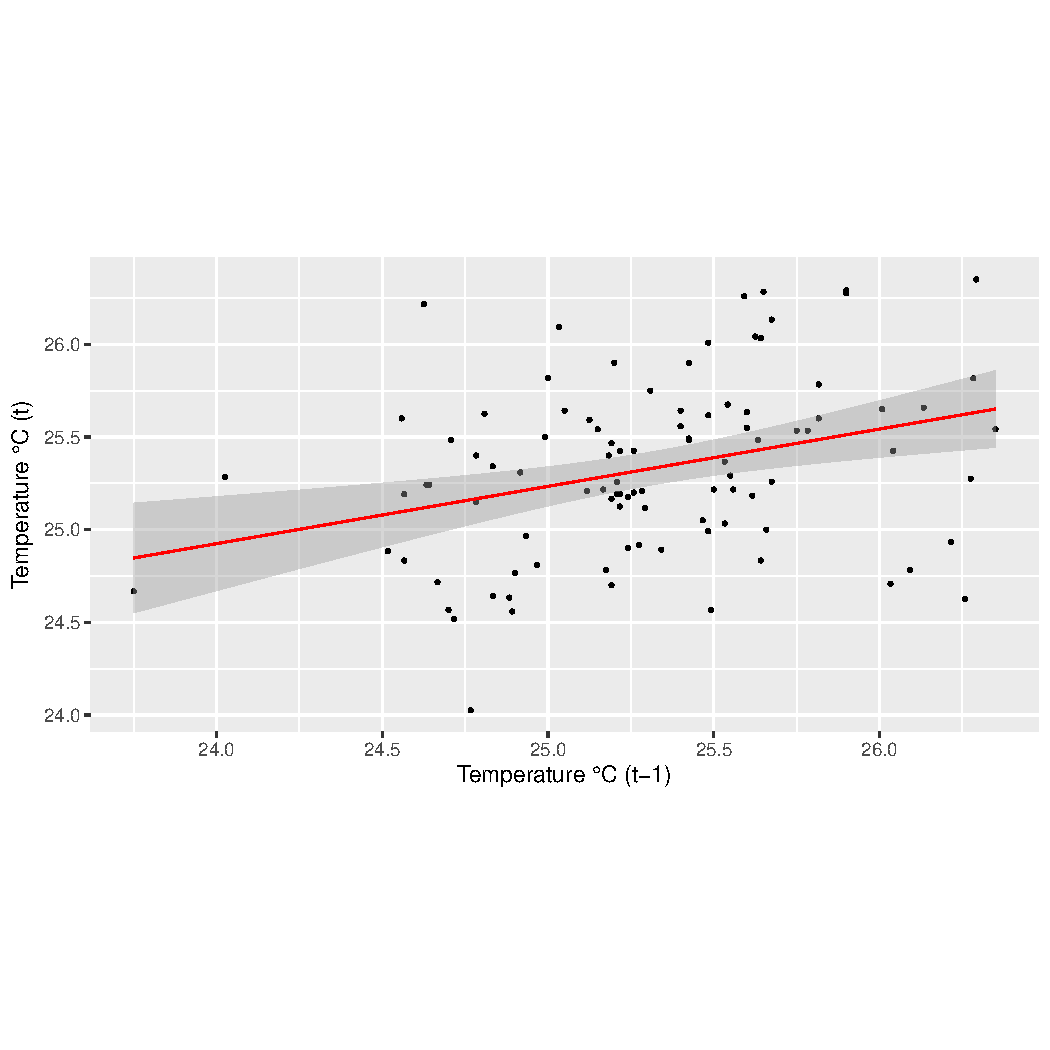
\includegraphics[width=1\textwidth]{../Results/AutoCorrScatter.pdf}
	\vspace{-30mm} % A global option would be better here
	\caption{Weather autocorrelation over the 20th century in Key West, Florida.}
	\vspace{-30mm} % A global option would be better here
	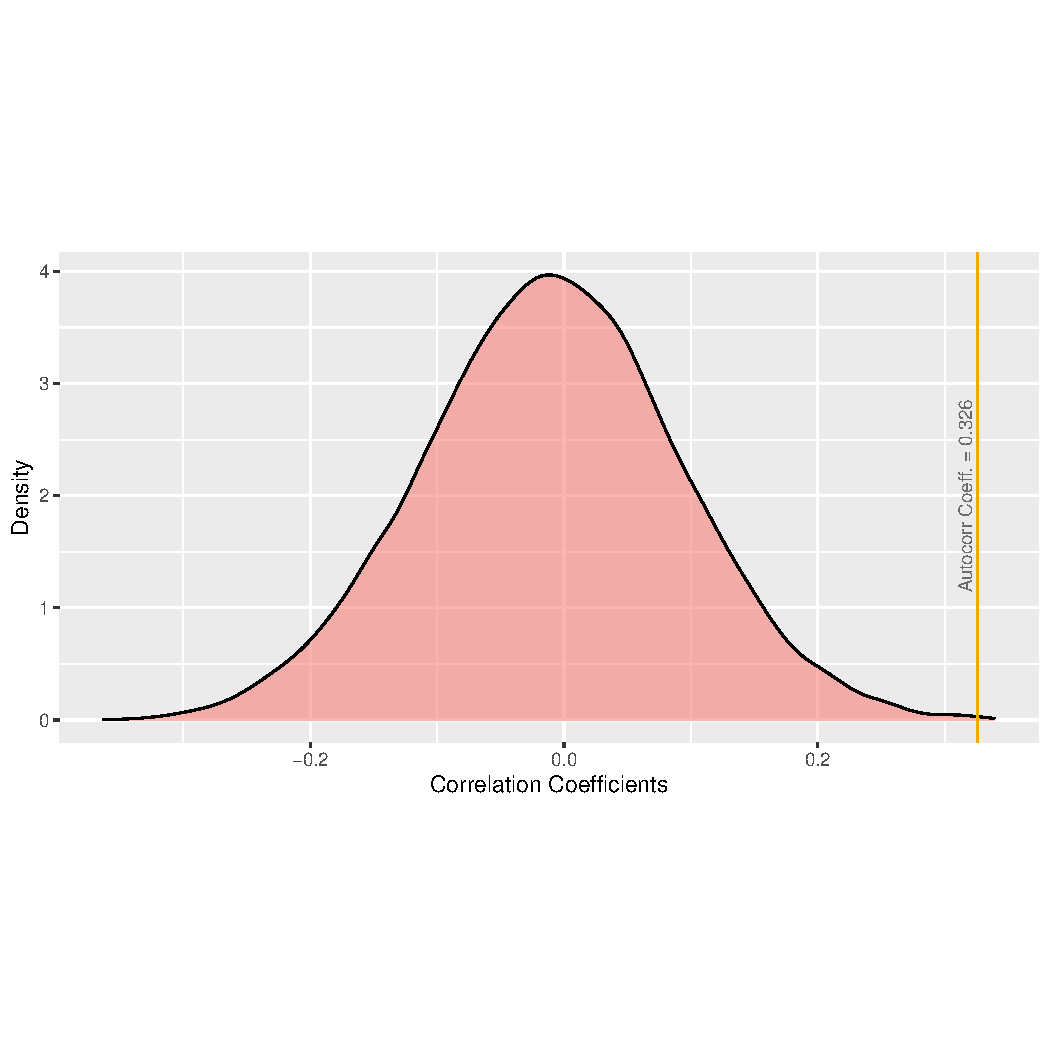
\includegraphics[width=1\textwidth]{../Results/AutoCorrDensity.pdf}
	\vspace{-30mm} % A global option would be better here
	\caption{Density plot of autocorrelation coefficients for 10,000 random permutations of the annual temperatures in the region over the century.}
    \end{figure}
    
	\section{Discussion}
	In conclusion, our results strongly indicate a positive autocorrelation between successive years across years in Key West, Florida ($r=0.326$), and that this autocorrelation is statistically significantly different from 0 ($p < 0.0005$).
	
	Opportunities for further investigation include comparing these findings with similar data from other regions to determine whether they constitute a localised or more general trend. Another possibility would be to investigate whether this data is better fit by a non-linear model.

\end{document}